\chapter{树}
\intro{树是无向图中最重要的一类——它是最"薄"的连通图，也是图论中应用最广泛的结构之一。任何连通无回路的无向图都称为树。}

\section{树的基本概念}

\subsection{树的定义}

\begin{mydefinition}{}
一个\textbf{无回路的连通无向图}称为\textbf{树}，通常记作 $T$。
\[
\boxed{\text{树} \;=\; \text{连通} \;+\; \text{无回路}}
\]
\end{mydefinition}

\begin{itemize}
    \item 树的边数恰好比顶点数少 $1$。
    \item 树是\textbf{极小连通图}：删去任意一条边，图就不再连通。
    \item 树是\textbf{极大无回路图}：添加任意一条边，图就产生回路。
\end{itemize}

\begin{center}
\begin{tikzpicture}[
    dmTreeNode/.style={circle, draw=green!50!black, fill=green!10, minimum size=9mm, inner sep=0pt},
    dmTreeEdge/.style={thick, draw=green!50!black}
]
% Example trees for n=1,2,3,4
% n=1
\node[dmTreeNode] (t1) at (0,0) {};
\node at (0, -0.7) {$n=1$};

% n=2
\node[dmTreeNode] (t2a) at (2,0) {};
\node[dmTreeNode] (t2b) at (3,0) {};
\draw[dmTreeEdge] (t2a) -- (t2b);
\node at (2.5, -0.7) {$n=2$};

% n=3 (path)
\node[dmTreeNode] (t3a) at (5,0) {};
\node[dmTreeNode] (t3b) at (6,0) {};
\node[dmTreeNode] (t3c) at (7,0) {};
\draw[dmTreeEdge] (t3a) -- (t3b) -- (t3c);
\node at (6, -0.7) {$n=3$};

% n=4 - path and star
\node[dmTreeNode] (t4pa) at (0,-3) {};
\node[dmTreeNode] (t4pb) at (1.2,-3) {};
\node[dmTreeNode] (t4pc) at (2.4,-3) {};
\node[dmTreeNode] (t4pd) at (3.6,-3) {};
\draw[dmTreeEdge] (t4pa) -- (t4pb) -- (t4pc) -- (t4pd);
\node at (1.8, -3.7) {$P_4$（路）};

\node[dmTreeNode] (t4sa) at (6,-4) {};
\node[dmTreeNode] (t4sb) at (5.4,-3) {};
\node[dmTreeNode] (t4sc) at (6,-3) {};
\node[dmTreeNode] (t4sd) at (6.6,-3) {};
\draw[dmTreeEdge] (t4sa) -- (t4sb);
\draw[dmTreeEdge] (t4sa) -- (t4sc);
\draw[dmTreeEdge] (t4sa) -- (t4sd);
\node at (6, -4.5) {$K_{1,3}$（星）};
\end{tikzpicture}
\end{center}

\subsection{树的六个等价条件}

\begin{myTheorem}{树的等价刻画}
设 $T$ 是 $n$ 阶无向简单图（$n \geq 1$），以下命题等价：
\end{myTheorem}

\begin{enumerate}
    \item $T$ 连通且无回路（树的原始定义）
    \item $T$ 无回路且有 $n-1$ 条边
    \item $T$ 连通且有 $n-1$ 条边
    \item $T$ 连通，但删去任一边后不再连通（极小连通图）
    \item $T$ 无回路，但添加任一边后恰有一个回路（极大无回路图）
    \item $T$ 中任意两顶点间有唯一简单路径
\end{enumerate}

\begin{center}
\begin{tikzpicture}[
    dmEquivNode/.style={rectangle, draw=blue!60, fill=blue!5, rounded corners, minimum width=3cm, minimum height=0.8cm, align=center},
    dmEquivArrow/.style={->, >=Stealth, thick, blue!60}
]
\node[dmEquivNode, fill=green!10, draw=green!50!black] (e1) at (0,4) {(1) 连通 + 无回路};
\node[dmEquivNode] (e2) at (3.5,4) {(2) 无回路 + $n-1$ 边};
\node[dmEquivNode] (e3) at (7,4)   {(3) 连通 + $n-1$ 边};
\node[dmEquivNode] (e6) at (0,1)   {(6) 唯一简单路径};
\node[dmEquivNode] (e5) at (3.5,1) {(5) 极大无回路};
\node[dmEquivNode] (e4) at (7,1)   {(4) 极小连通};

\draw[dmEquivArrow] (e1) -- (e2);
\draw[dmEquivArrow] (e2) -- (e3);
\draw[dmEquivArrow] (e3) -- (e4);
\draw[dmEquivArrow] (e4) -- (e5);
\draw[dmEquivArrow] (e5) -- (e6);
\draw[dmEquivArrow] (e6) -- (e1);
\end{tikzpicture}
\end{center}

\begin{proof}
我们证明 $(1)\Rightarrow(2)\Rightarrow(3)\Rightarrow(4)\Rightarrow(5)\Rightarrow(6)\Rightarrow(1)$。

\medskip
\textbf{(1)$\Rightarrow$(2)}：对 $n$ 归纳。$n=1$ 时边数为 $0 = 1-1$。假设对少于 $n$ 个顶点的树成立。在 $T$ 中任取一边 $e$，删去 $e$ 后图分为两个连通分支 $T_1, T_2$，分别有 $n_1, n_2$ 个顶点（$n_1+n_2=n$）。由归纳假设，边数分别为 $n_1-1, n_2-1$，故总边数 $m = (n_1-1)+(n_2-1)+1 = n-1$。

\textbf{(2)$\Rightarrow$(3)}：设 $T$ 有 $c$ 个连通分支，每个分支是树，故边数为 $n_i-1$。总边数 $m = \sum (n_i-1) = n - c$。已知 $m = n-1$，得 $c=1$，即 $T$ 连通。

\textbf{(3)$\Rightarrow$(4)}：$T$ 连通且有 $n-1$ 条边。任删一边 $e$，得 $T-e$（仍有 $n$ 个顶点，$n-2$ 条边）。由连通图的边数下界，$T-e$ 不可能连通，故 $T$ 极小连通。

\textbf{(4)$\Rightarrow$(5)}：先证无回路：若 $T$ 有回路 $C$，删去 $C$ 上任一边 $e$，$T-e$ 仍连通，矛盾。再证极大无回路：任加一边 $e=(u,v)$，由于 $T$ 连通，$u$ 和 $v$ 间已有路径 $P$，$P\cup\{e\}$ 形成回路。

\textbf{(5)$\Rightarrow$(6)}：先证连通性：若 $T$ 不连通，则存在分属不同分支的顶点 $u,v$，添加边 $(u,v)$ 不会产生回路，矛盾。再证唯一性：$T$ 连通保证了任意两点间至少有一条路径。若有两条不同路径，则它们的对称差含有回路，与无回路矛盾。

\textbf{(6)$\Rightarrow$(1)}：连通性显然。无回路：若存在回路 $C$，则 $C$ 上任意相邻两顶点间的边和回路其余部分给出两条不同路径，矛盾。
\end{proof}

\subsection{树叶与森林}

\begin{mydefinition}{}
\begin{itemize}
    \item 树中度数为 $1$ 的顶点称为\textbf{树叶}。度数为 $0$ 的孤立顶点也视为树叶（在平凡树中）。
    \item 度 $\geq 2$ 的顶点称为\textbf{分支结点}（内结点）。
    \item 一个无回路（但可以不连通）的无向图称为\textbf{森林}。森林的每个连通分支都是树。
    \item 若森林有 $n$ 个顶点、$c$ 个连通分支，则边数 $m = n - c$。
\end{itemize}
\end{mydefinition}

\begin{myTheorem}{树叶数量}
任何非平凡的树（$n \geq 2$）至少有 \textbf{2 片树叶}。
\end{myTheorem}

\begin{proof}
设树 $T$ 有 $n$ 个顶点，$m = n-1$ 条边。设树叶数为 $k$，非树叶数为 $n-k$。由握手定理：
\[
2m = \sum_{v\in V} \deg(v) \geq k \cdot 1 + (n-k) \cdot 2 = 2n - k
\]
代入 $m = n-1$ 得：$2(n-1) \geq 2n - k$，即 $2n-2 \geq 2n-k$，故 $k \geq 2$。
\end{proof}

\section{生成树}

\subsection{定义与存在性}

\begin{mydefinition}{}
设 $G$ 是连通无向图。$G$ 的一个\textbf{生成树}是 $G$ 的一个生成子图 $T$，且 $T$ 是树。等价地说，从 $G$ 中删去一些边，使得剩下的图连通且无回路。
\end{mydefinition}

\begin{myTheorem}{存在性}
每个连通无向图至少有一棵生成树。
\end{myTheorem}

构造方法：\textbf{破圈法}（反复找回路并删去一条边）或\textbf{避圈法}（从空边集开始，每次选取一条不产生回路的新边加入，直到选满 $n-1$ 条边）。

\subsection{最小生成树 (MST)}

\begin{mydefinition}{}
给定连通带权无向图 $G=(V,E,w)$，$G$ 的\textbf{最小生成树}是 $G$ 的一棵生成树 $T$，使得总权值 $w(T) = \sum_{e \in E(T)} w(e)$ 在所有生成树中最小。
\end{mydefinition}

\subsubsection{Prim 算法}

\begin{myalgorithm}{Prim 算法（$O(n^2)$ 朴素实现）}
\begin{enumerate}
    \item 任选起点 $v_0 \in V$，设 $S = \{v_0\}$，$T = \emptyset$。
    \item 重复 $n-1$ 次：在所有跨 $S$ 和 $V \setminus S$ 的边中，选权值最小的边 $e = (u,v)$（$u \in S, v \in V\setminus S$），将 $e$ 加入 $T$，将 $v$ 加入 $S$。
    \item 返回 $T$。
\end{enumerate}
\end{myalgorithm}

\begin{center}
\begin{tikzpicture}[
    dmMSTNode/.style={circle, draw=blue!60, fill=blue!10, minimum size=9mm, inner sep=0pt},
    dmMSTSelected/.style={circle, draw=red!60, fill=red!15, minimum size=9mm, inner sep=0pt},
    dmMSTEdge/.style={thick, draw=gray!40},
    dmMSTInTree/.style={thick, draw=red!70, >={Stealth}}
]
% Prim algorithm step-by-step visualization
\node[dmMSTSelected] (pa) at (0,2)   {A};
\node[dmMSTNode] (pb) at (2,3)   {B};
\node[dmMSTNode] (pc) at (4,2)   {C};
\node[dmMSTNode] (pd) at (4,0)   {D};
\node[dmMSTNode] (pe) at (2,-1)  {E};
\node[dmMSTNode] (pf) at (0,0)   {F};

\draw[dmMSTEdge] (pa) -- node[above left] {6} (pb);
\draw[dmMSTEdge] (pa) -- node[above] {1} (pc);
\draw[dmMSTEdge] (pa) -- node[below left] {5} (pf);
\draw[dmMSTEdge] (pb) -- node[right] {5} (pc);
\draw[dmMSTEdge] (pb) -- node[below right] {3} (pd);
\draw[dmMSTEdge] (pb) -- node[left] {6} (pe);
\draw[dmMSTEdge] (pc) -- node[right] {5} (pd);
\draw[dmMSTEdge] (pc) -- node[above right] {4} (pe);
\draw[dmMSTEdge] (pc) -- node[above left] {2} (pf);
\draw[dmMSTEdge] (pd) -- node[right] {6} (pe);
\draw[dmMSTEdge] (pd) -- node[below] {6} (pf);
\draw[dmMSTEdge] (pe) -- node[below] {6} (pf);

% Highlight selected edges in the MST: A-C, C-F, C-E, E-D, E-B (example weights)
\draw[dmMSTInTree, red!70] (pa) -- (pc);
\draw[dmMSTInTree, red!70] (pc) -- (pf);
\draw[dmMSTInTree, red!70] (pc) -- (pe);
\draw[dmMSTInTree, red!70] (pe) -- (pd);
\draw[dmMSTInTree, red!70] (pe) -- (pb);

\node[dmMSTSelected] at (pa) {A};
\node[dmMSTSelected] at (pc) {C};
\node[dmMSTSelected] at (pf) {F};
\node[dmMSTSelected] at (pe) {E};
\node[dmMSTSelected] at (pd) {D};
\node[dmMSTSelected] at (pb) {B};

\node at (2, -2.0) {\fangsong Prim 算法示例：从 A 开始，红色边构成 MST，总权值 = $1+2+4+6+3=16$};
\end{tikzpicture}
\end{center}

\subsubsection{Kruskal 算法}

\begin{myalgorithm}{Kruskal 算法（$O(m \log m)$）}
\begin{enumerate}
    \item 将所有边按权值从小到大排序。
    \item 初始化并查集：每个顶点自成一个集合。
    \item 按排序顺序遍历每条边 $e=(u,v)$：若 $u$ 和 $v$ 不在同一集合，则选取 $e$，合并 $u$ 和 $v$ 所在的集合。
    \item 当选取了 $n-1$ 条边时停止。
\end{enumerate}
\end{myalgorithm}

\subsection{Cayley 定理}

\begin{myTheorem}{Cayley 定理}
$n$ 个标号顶点的完全图 $K_n$ 中，不同生成树的个数为：
\[
\boxed{T(n) = n^{n-2}}
\]
\end{myTheorem}

例如 $n=3$：$3^1 = 3$；$n=4$：$4^2 = 16$。此定理可通过 Pr\"ufer 编码证明：Pr\"ufer 序列与标号树一一对应，而 Pr\"ufer 序列的每一位可取 $1$ 到 $n$ 的任意值，长度为 $n-2$，故有 $n^{n-2}$ 种。

\section{有根树与二叉树}

\subsection{有根树}

\begin{mydefinition}{}
选定树的一个顶点作为\textbf{根}，并规定所有边的方向为远离根的方向，得到的向树称为\textbf{有根树}。
\end{mydefinition}

\begin{itemize}
    \item 根画在最上方，边朝下。
    \item 顶点 $v$ 的\textbf{深度}是从根到 $v$ 的唯一路径长度（边数）。
    \item 树的\textbf{高度}是最大深度。
    \item 父结点、子结点、兄弟、祖先、后代、子树——参见图例。
\end{itemize}

\begin{center}
\begin{tikzpicture}[
    dmRootNode/.style={circle, draw=red!60, fill=red!10, minimum size=8mm, inner sep=0pt},
    dmRChildNode/.style={circle, draw=blue!60, fill=blue!10, minimum size=8mm, inner sep=0pt},
    dmRLeafNode/.style={circle, draw=green!40!black, fill=green!10, minimum size=8mm, inner sep=0pt},
    dmREdge/.style={thick, ->, >=Stealth},
    level 1/.style={sibling distance=2.2cm},
    level 2/.style={sibling distance=1.2cm},
    level 3/.style={sibling distance=0.8cm}
]
\node[dmRootNode] {\small 根}
    child { node[dmRChildNode] {\small 内}
        child { node[dmRLeafNode] {\small 叶}
            child { node[dmRLeafNode] {\small 叶} }
        }
        child { node[dmRLeafNode] {\small 叶} }
    }
    child { node[dmRChildNode] {\small 内}
        child { node[dmRLeafNode] {\small 叶} }
    };

\foreach \from/\to/\label in {}
    \path (\from) edge[dmREdge] (\to);

\node at (0, -5.5) {\fangsong 有根树结构：根（红色）、内结点（蓝色）、树叶（绿色）};
\end{tikzpicture}
\end{center}

\subsection{$m$ 叉树}

\begin{mydefinition}{}
有根树中，每个顶点最多有 $m$ 个子结点的称为 \textbf{$m$ 叉树}。
\begin{itemize}
    \item \textbf{正则 $m$ 叉树}：每个分支结点恰好有 $m$ 个子结点。
    \item \textbf{完全 $m$ 叉树}：树叶都在同一层，且每个内结点恰有 $m$ 个子结点。
\end{itemize}
\end{mydefinition}

\begin{myTheorem}{正则 $m$ 叉树的树叶与分支结点关系}
设 $i$ 为分支结点数，$l$ 为树叶数，则
\[
l = (m-1)i + 1
\]
\end{myTheorem}

\subsection{二叉树}

\begin{mydefinition}{}
一棵二叉树是有限个顶点的集合，它或者为空，或者由一个根顶点和两棵互不相交的、分别称为\textbf{左子树}和\textbf{右子树}的二叉树组成。
\end{mydefinition}

\begin{remark}
二叉树不是普通的 2 叉树。在二叉树中，子树有\textbf{左右之分}，即使一个子树为空。在普通的有根树中，子结点是无序的。
\end{remark}

\textbf{二叉树的基本性质}：

\begin{enumerate}
    \item 二叉树第 $i$ 层（$i \geq 1$）最多有 $2^{i-1}$ 个结点。
    \item 深度为 $k$ 的二叉树最多有 $2^k-1$ 个结点。
    \item 对任意二叉树，若度为 2 的结点个数为 $n_2$，树叶个数为 $n_0$，则
    \[
    \boxed{n_0 = n_2 + 1}
    \]
\end{enumerate}

\begin{proof}
设有 $n$ 个结点，$m$ 条边，$n_1$ 个度为 1 的结点。则 $n = n_0 + n_1 + n_2$。所有结点度数之和等于边数的 2 倍：$n_1 + 2n_2 = 2m$。在树中 $m = n - 1$，代入得 $n_1 + 2n_2 = 2(n_0 + n_1 + n_2 - 1)$。化简得 $2n_0 = n_1 + 2$，又 $n_1 + 2n_2 = 2(n - 1)$，可以推出 $n_0 = n_2 + 1$。
\end{proof}

\subsection{二叉树的遍历}

\begin{center}
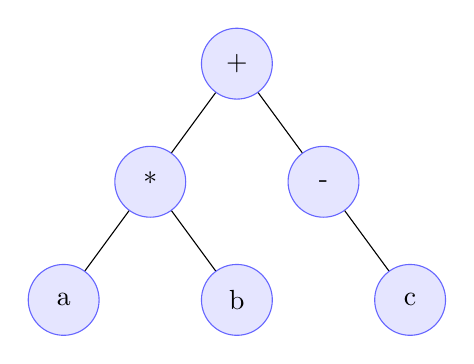
\begin{tikzpicture}[
    dmBTNode/.style={circle, draw=blue!60, fill=blue!10, minimum size=9mm, inner sep=0pt},
    dmBTEdge/.style={thick},
    level distance=1.5cm,
    sibling distance=2.2cm
]
\node[dmBTNode] {+}
    child { node[dmBTNode] {*}
        child { node[dmBTNode] {a} }
        child { node[dmBTNode] {b} }
    }
    child { node[dmBTNode] {-}
        child [missing]
        child { node[dmBTNode] {c} }
    };
\end{tikzpicture}
\end{center}

\vspace{0.3cm}

\begin{center}
\begin{tabular}{c|c|c}
\hline
\textbf{遍历方式} & \textbf{次序} & \textbf{结果} \\
\hline
前序遍历 (DLR) & 根 $\to$ 左 $\to$ 右 & $+\;*\;a\;b\;-\;c$ （波兰表示法）\\
中序遍历 (LDR) & 左 $\to$ 根 $\to$ 右 & $a\;*\;b\;+\;-\;c$ 需加括号 \\
后序遍历 (LRD) & 左 $\to$ 右 $\to$ 根 & $a\;b\;*\;c\;-\;+$ （逆波兰表示法）\\
\hline
\end{tabular}
\end{center}

\begin{myTheorem}{遍历序列重建二叉树}
\begin{itemize}
    \item \textbf{前序 + 中序} 可以唯一确定一棵二叉树。
    \item \textbf{后序 + 中序} 可以唯一确定一棵二叉树。
    \item 仅有前序和后序\textbf{无法}唯一确定二叉树。
\end{itemize}
\end{myTheorem}

\section{哈夫曼树与哈夫曼编码}

\subsection{哈夫曼树（最优二叉树）}

\begin{mydefinition}{}
设二叉树有 $n$ 个带权树叶，权值分别为 $w_1, w_2, \dots, w_n$，树叶的路径长度（从根到树叶的边数）为 $l_1, l_2, \dots, l_n$。则二叉树的\textbf{带权路径长度 (WPL)} 定义为：
\[
\boxed{\text{WPL} = \sum_{i=1}^{n} w_i \cdot l_i}
\]
\end{mydefinition}

\begin{mydefinition}{}
给定一组权值，使得 WPL 最小的二叉树称为\textbf{最优二叉树}或\textbf{哈夫曼树}。
\end{mydefinition}

\begin{myalgorithm}{哈夫曼算法（$O(n \log n)$）}
\begin{enumerate}
    \item 构造 $n$ 棵单结点二叉树（每个结点携带一个权值），放入集合 $F$。
    \item 重复 $n-1$ 次：
    \begin{enumerate}
        \item 从 $F$ 中取出两棵根权值最小的树作为左右子树。
        \item 构造一棵新二叉树，新树的根权值为左右子树根权值之和。
        \item 将新树加入 $F$。
    \end{enumerate}
    \item $F$ 中只剩一棵树，即为哈夫曼树。
\end{enumerate}
\end{myalgorithm}

\begin{center}
\begin{tikzpicture}[
    dmHuffNode/.style={circle, draw=orange!70, fill=orange!10, minimum size=9mm, inner sep=0pt},
    dmHuffLeaf/.style={circle, draw=green!40!black, fill=green!10, minimum size=9mm, inner sep=0pt},
    dmHuffEdge0/.style={thick, draw=blue!60},
    dmHuffEdge1/.style={thick, draw=red!60},
    level distance=1.6cm,
    sibling distance=2.5cm
]
\node[dmHuffNode] {\small 100}
    child {
        node[dmHuffNode] {\small 45}
        child {
            node[dmHuffNode] {\small 25}
            child { node[dmHuffLeaf] {\small 12} edge from parent[dmHuffEdge0] node[left] {0} }
            child { node[dmHuffLeaf] {\small 13} edge from parent[dmHuffEdge1] node[right] {1} }
            edge from parent[dmHuffEdge0] node[left] {0}
        }
        child {
            node[dmHuffNode] {\small 20}
            child { node[dmHuffLeaf] {\small 9} edge from parent[dmHuffEdge0] node[left] {0} }
            child { node[dmHuffLeaf] {\small 11} edge from parent[dmHuffEdge1] node[right] {1} }
            edge from parent[dmHuffEdge1] node[right] {1}
        }
    }
    child {
        node[dmHuffNode] {\small 55}
        child {
            node[dmHuffNode] {\small 30}
            child { node[dmHuffLeaf] {\small 14} edge from parent[dmHuffEdge0] node[left] {0} }
            child { node[dmHuffLeaf] {\small 16} edge from parent[dmHuffEdge1] node[right] {1} }
            edge from parent[dmHuffEdge0] node[left] {0}
        }
        child {
            node[dmHuffLeaf] {\small 25}
            edge from parent[dmHuffEdge1] node[right] {1}
        }
    };

\node at (0, -6.5) {\fangsong 哈夫曼树示例（权值 9, 11, 12, 13, 14, 16, 25）：左分支标记 0，右分支标记 1};
\end{tikzpicture}
\end{center}

\subsection{哈夫曼编码}

\begin{mydefinition}{}
一个编码集合，其中没有任何一个编码是另一个编码的前缀，称为\textbf{前缀码}。
\end{mydefinition}

\textbf{构造方法}：
\begin{enumerate}
    \item 以字符频率为权值构建哈夫曼树。
    \item 左分支标记为 \texttt{0}，右分支标记为 \texttt{1}。
    \item 每个字符的编码为从根到该字符树叶的路径标记序列。
\end{enumerate}

哈夫曼编码是\textbf{最优前缀码}——对于给定的字符频率，其平均码长最短。

\section{编程实现}

\begin{mycode}{哈夫曼编码}
\begin{lstlisting}[language=Python]
import heapq

class HuffNode:
    def __init__(self, ch, freq):
        self.ch = ch
        self.freq = freq
        self.left = self.right = None
    def __lt__(self, other):
        return self.freq < other.freq

def build_huffman(freq_map):
    heap = [HuffNode(ch, f) for ch, f in freq_map.items()]
    heapq.heapify(heap)
    while len(heap) > 1:
        left = heapq.heappop(heap)
        right = heapq.heappop(heap)
        parent = HuffNode('', left.freq + right.freq)
        parent.left, parent.right = left, right
        heapq.heappush(heap, parent)
    return heap[0]

def encode(root, code='', code_map=None):
    if code_map is None:
        code_map = {}
    if root:
        if not root.left and not root.right:
            code_map[root.ch] = code
        encode(root.left, code + '0', code_map)
        encode(root.right, code + '1', code_map)
    return code_map

freq = {'a': 5, 'b': 9, 'c': 12, 'd': 13, 'e': 16, 'f': 45}
root = build_huffman(freq)
codes = encode(root)
for ch, code in codes.items():
    print(f"{ch}: {code}")
\end{lstlisting}
\end{mycode}

\begin{mycode}{Prim 与 Kruskal 算法}
\begin{lstlisting}[language=Python]
# Prim 算法
def prim(graph, n):
    INF = float('inf')
    dist = [INF] * n
    visited = [False] * n
    dist[0] = 0
    total = 0
    for _ in range(n):
        u = min((j for j in range(n) if not visited[j]),
                key=lambda j: dist[j], default=-1)
        if u == -1:
            break
        visited[u] = True
        total += dist[u]
        for v in range(n):
            if not visited[v] and graph[u][v] < dist[v]:
                dist[v] = graph[u][v]
    return total

# Kruskal 算法
class DSU:
    def __init__(self, n):
        self.p = list(range(n))
        self.r = [0] * n
    def find(self, x):
        if self.p[x] != x:
            self.p[x] = self.find(self.p[x])
        return self.p[x]
    def union(self, x, y):
        x, y = self.find(x), self.find(y)
        if x == y: return
        if self.r[x] < self.r[y]:
            x, y = y, x
        self.p[y] = x
        if self.r[x] == self.r[y]:
            self.r[x] += 1

def kruskal(edges, n):
    edges.sort(key=lambda e: e[2])
    dsu = DSU(n)
    total = 0
    for u, v, w in edges:
        if dsu.find(u) != dsu.find(v):
            dsu.union(u, v)
            total += w
    return total
\end{lstlisting}
\end{mycode}

\begin{mycode}{二叉树遍历}
\begin{lstlisting}[language=Python]
from collections import deque

class TreeNode:
    def __init__(self, val, left=None, right=None):
        self.val = val
        self.left = left
        self.right = right

def preorder(root):
    return [root.val] + preorder(root.left) + preorder(root.right) if root else []

def inorder(root):
    return inorder(root.left) + [root.val] + inorder(root.right) if root else []

def postorder(root):
    return postorder(root.left) + postorder(root.right) + [root.val] if root else []

def level_order(root):
    if not root:
        return []
    res, q = [], deque([root])
    while q:
        node = q.popleft()
        res.append(node.val)
        if node.left:  q.append(node.left)
        if node.right: q.append(node.right)
    return res

# 示例
root = TreeNode('+',
    TreeNode('*', TreeNode('a'), TreeNode('b')),
    TreeNode('-', None, TreeNode('c')))
print(f"前序: {''.join(preorder(root))}")
print(f"中序: {''.join(inorder(root))}")
print(f"后序: {''.join(postorder(root))}")
\end{lstlisting}
\end{mycode}

\section{本章小结}

\begin{myTheorem}{树的核心知识体系}
\[
\begin{array}{c|l}
\hline
\textbf{概念} & \textbf{核心要点} \\
\hline
\text{树} & n\text{ 顶点，}n-1\text{ 边的连通无回路图。六个等价条件。} \\
\text{树叶} & \text{非平凡树至少 2 片树叶。} \\
\text{生成树} & \text{连通图的极小连通生成子图。} \\
\text{MST} & \text{Prim }O(n^2)\text{ 稠密图，Kruskal }O(m\log m)\text{ 稀疏图。} \\
\text{Cayley 定理} & n\text{ 标号顶点的不同树有 }n^{n-2}\text{ 个。} \\
\text{二叉树性质} & n_0=n_2+1\text{，第 }i\text{ 层最多 }2^{i-1}\text{ 个结点。} \\
\text{遍历} & \text{前序/中序/后序 (DLR/LDR/LRD)。前中或后中可重建二叉树。} \\
\text{哈夫曼树} & \text{带权路径长度最小的二叉树，}O(n\log n)\text{ 构建。} \\
\text{哈夫曼编码} & \text{最优前缀码，平均码长最短。} \\
\hline
\end{array}
\]
\end{myTheorem}
